\ifx\wholebook\relax \else

\documentclass[b5paper]{ctexart}
\usepackage[nomarginpar
  %, margin=.5in
]{geometry}

\addtolength{\oddsidemargin}{-0.05in}
\addtolength{\evensidemargin}{-0.05in}
\addtolength{\textwidth}{0.1in}

\usepackage[cn]{../prelude}

\setcounter{page}{1}

\begin{document}

\title{复数}

\author{刘新宇
\thanks{{\bfseries 刘新宇} \newline
  Email: liuxinyu99@hotmail.com \newline}
  }

\maketitle
\fi

\markboth{复数}{数的旅程}

\ifx\wholebook\relax
\chapter{复数}
\fi

%% On earth there is nothing great but man; and in man there is nothing great but mind.
\epigraph{地球上最伟大的是人,人之中最伟大的是心灵}{威廉·汉密尔顿}

读过金庸武侠小说的读者一定对“华山论剑”津津乐道。天下武林中的顶级高手约定在华山比武论剑。大家各自身怀秘不外传的绝世武功,通过比武确定谁是真正的天下武功第一。十六世纪的意大利也上演了精彩的华山论剑。只不过没有刀光剑影、没有拳脚身法,而是一场关于数学与荣誉的挑战。1535年2月13日深夜,塔尔塔利亚在威尼斯的家中踱来踱去,为即将到来的挑战苦思冥想。文艺复兴时期的意大利,学着剪经常进行骑士般的公开挑战。这种挑战并不使用刀剑或者火枪进行决斗,双方各自向对方提出同等数目的数学或科学题目,并在规定的时间内作答。正确答出多的人获胜。胜利的一方赢得荣誉或一定数目的奖金。这种一对一的“单挑”发生在知名学者之间,通常在大教堂这类城市公共场所进行,引起众人的围观。有时甚至市长或者贵族也会前来观看,因而使得胜负具有非常的意义,影响双方的社会地位、学术评价甚至职业发展。

例如1225年,神圣罗马帝国皇帝腓特烈二世在西西里行宫接见了斐波那契。宫廷学者看不起商人出身的数学家,于是向斐波那契发起了挑战。斐波那契成功解决了全部问题,为自己赢得了荣誉。这些题目中包含了一道一元三次方程\footnote{当时还没有代数符号,是用文字描述的,如:找到一个数,其立方加上其平方的两倍再加上其十倍是二十。}:\[x^3 + 2x^2 + 10x = 20\]

斐波那契使用古巴比伦的60进制数值解法给出了正确答案:
\[
1^022^{I}7^{II}42^{III}33^{IV}4^{V}40^{VI} = 1 + \frac{22}{60} + \frac{7}{60^2} + \frac{42}{60^3} + \dotsb
\]

相当于十进制小数1.3688081075,精确到了小数点后9位。这种公开挑战也造成了一种奇特现象:学者们把自己的研究成果视为高度机密。因为这样可以使得他在与别人的挑战中获得优势。一旦泄露,对方就能解出自己提出的问题。学者们在生前不发表自己的成果,而是在死前传给自己信任的门生。这在“不发表就发霉”的今天是很难理解的\cite{HanXuetao2012}。

塔尔塔利亚面临的挑战就是关于三次方程的,对手名叫费奥尔\footnote{安东尼奥・马里亚・费奥尔,Antonio Maria Fior}。尽管古巴比伦人在公元前2500左右就掌握了一元二次方程的解法,但人们在接下来的4000多年一直没有突破一般三次方程的解法。人们并不满足于斐波那契的数值解法,而希望得到如二次方程那样的求根公式。所谓\underdot{一般}是指形如$ax^3 + bx^2 + cx + d = 0$的三次方程,简单的特殊三次方程,如$x^3 = a$自然容易解出一个\footnote{另外两个根是复数:$\dfrac{-1 \pm i\sqrt{3}}{2}\sqrt[3]{a}$}根$x = \sqrt[3]{a}$。塔尔塔利亚经过自己的努力,独立发现了形如$x^3 + ax^2 = b$这种特殊三次方程的解。

\begin{figure}[htbp]
  \centering
  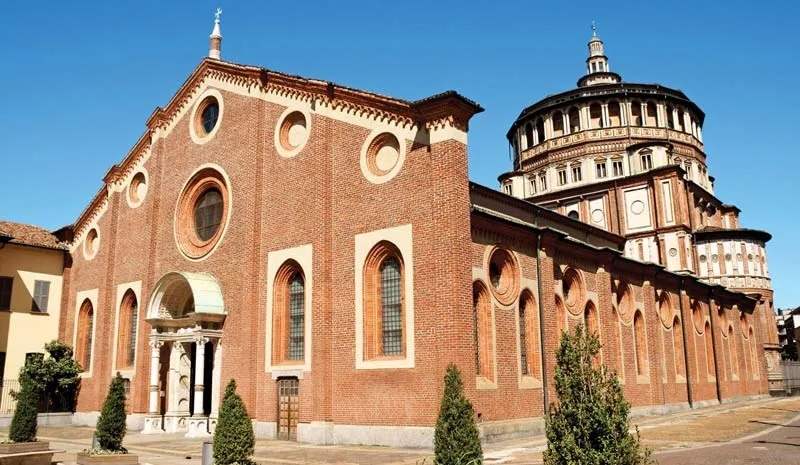
\includegraphics[scale=0.33]{img/churchmilan}
  \caption{米兰圣母玛丽亚感恩大教堂}
 \label{fig:church-Milan}
\end{figure}

%% del Ferro:德尔・费罗(意大利数学家尼科洛・德尔・费罗,Niccolò del Ferro,15 世纪末至 16 世纪初,首次解出一元三次方程的一类特殊情况)
%% Fior:费奥尔(意大利数学家安东尼奥・马里亚・费奥尔,Antonio Maria Fior,16 世纪,曾与塔尔塔利亚就三次方程解法展开竞赛)
%% Ferrari:费拉里(意大利数学家洛多维科・费拉里,Lodovico Ferrari,16 世纪,在卡尔达诺指导下首次解出一元四次方程)

\section{三次方程}
解三次方程的历史

\section{佚名数学家}
\subsection{复数的几何意义和运算法则}
\subsection{匿名作者阿尔冈}
\subsection{代数基本定理}

\section{e的传奇}
\subsection{e的诞生}
\subsection{最美公式}

\section{新世界的大门}
\subsection{小试牛刀}
麦钦公式、正五边形作图
\subsection{费马大定理与高斯整数}
\subsection{抽象的数}
理想数
\subsection{新数的构造-代数数}

\ifx\wholebook\relax \else
\section{参考答案}
\shipoutAnswer

\begin{thebibliography}{99}
\subimport{inc/}{bib-zh-cn}
\end{thebibliography}

\expandafter\enddocument
\fi
